\chapter{Le titre du chapitre}

\section{Le titre de la section qui va bien}

\subsection{Titre de la sous section}

Exemple de code .
\lstset{language=HTML}
\begin{lstlisting}[label=some-css,caption=Some Html]
<style>
.header {
	background:#333;
	height:123px;

}
</style>

\end{lstlisting}
\lstset{language=PHP}
\begin{lstlisting}[label=some-php,caption=Some Php]
<?php
public class maClasse{
	public maFonction()
	{
		$maVar = new String("hello world");	
	}
}
?>

\end{lstlisting}
%$
\lstset{language=JavaScript}
\begin{lstlisting}[label=some-js,caption=Some JavaScript]

var mavar = new String('polop');
alert("hello world");
return false;

\end{lstlisting}

\lstset{language=SQL}
\begin{lstlisting}[label=some-sql,caption=Some SQL]

SELECT * FROM page WHERE id='1';

\end{lstlisting}

%-- Note de bas de page sur les stades
\protect\footnote{Par exemple, on peut faire un pied de page :
\begin{itemize}
\item avec une liste à puces ;
\item avec une liste à puces ;
\item avec une liste à puces.
\end{itemize}
}
%-- Fin Note de bas de page sur les stades

Ici du texte et du blabla, ce que l'on veut dire et écrire. A remplacer. Ici du texte et du blabla, ce que l'on veut dire et écrire. A remplacer. Ici du texte et du blabla, ce que l'on veut dire et écrire. A remplacer. Ici du texte et du blabla, ce que l'on veut dire et écrire. A remplacer. Ici du texte et du blabla, ce que l'on veut dire et écrire. A remplacer. Ici du texte et du blabla, ce que l'on veut dire et écrire. A remplacer.

\begin{itemize}
\item avec une liste à puces ;
\item avec une liste à puces ;
\item avec une liste à puces.
\end{itemize}

Ici du texte et du blabla, ce que l'on veut dire et écrire. A remplacer. Ici du texte et du blabla, ce que l'on veut dire et écrire. A remplacer. Ici du texte et du blabla, ce que l'on veut dire et écrire. A remplacer. Ici du texte et du blabla, ce que l'on veut dire et écrire. A remplacer. Ici du texte et du blabla, ce que l'on veut dire et écrire. A remplacer. Ici du texte et du blabla, ce que l'on veut dire et écrire. A remplacer.

\subsubsection{Titre de la sous sous section}

Ici du texte et du blabla, ce que l'on veut dire et écrire. A remplacer. Ici du texte et du blabla, ce que l'on veut dire et écrire. A remplacer. Ici du texte et du blabla, ce que l'on veut dire et écrire. A remplacer. Ici du texte et du blabla, ce que l'on veut dire et écrire. A remplacer. Ici du texte et du blabla, ce que l'on veut dire et écrire. A remplacer. Ici du texte et du blabla, ce que l'on veut dire et écrire. A remplacer.

%exemple d'image
\begin{figure}[!ht]
\centering
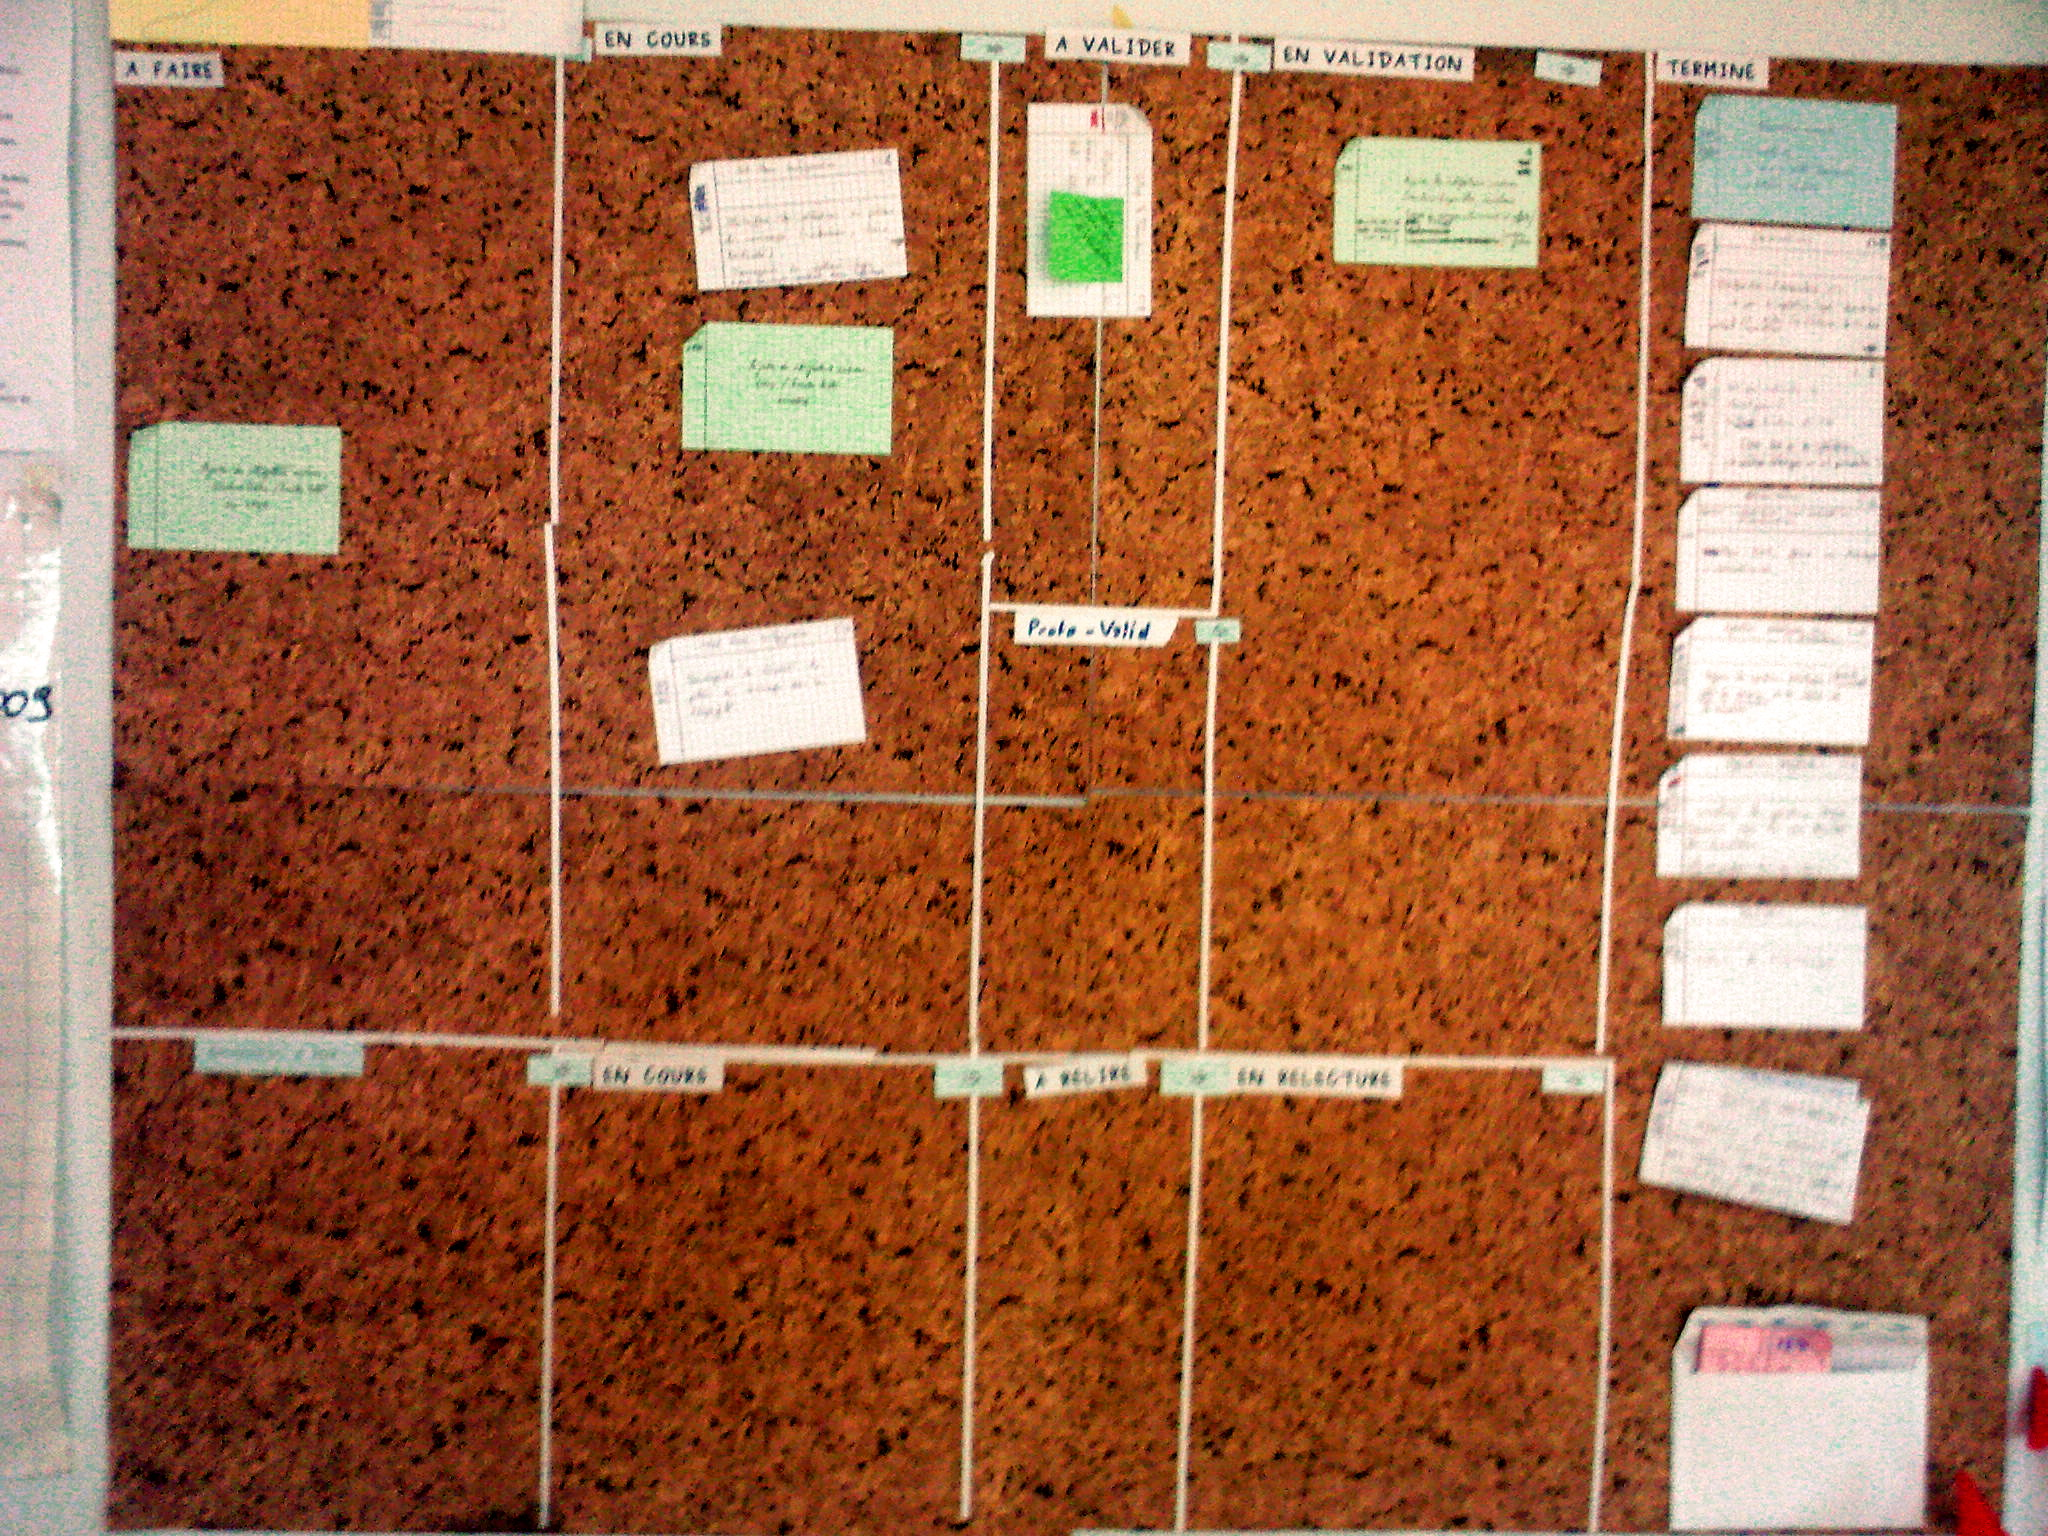
\includegraphics[width=.55\textwidth]{img/SP_A0183.jpg}
\caption{Image sample}
\label{figure:sampe}
\end{figure}

Ici du texte et du blabla, ce que l'on veut dire et écrire. A remplacer. Ici du texte et du blabla, ce que l'on veut dire et écrire. A remplacer. Ici du texte et du blabla, ce que l'on veut dire et écrire. A remplacer. Ici du texte et du blabla, ce que l'on veut dire et écrire. A remplacer. Ici du texte et du blabla, ce que l'on veut dire et écrire. A remplacer. Ici du texte et du blabla, ce que l'on veut dire et écrire. A remplacer.

\subsubsection{Titre de la sous sous section}

Exemple de tableau
\begin{table}[!ht]
	\caption{\label{tableau:evolPratXP}Evolution des pratiques XP au cours du stage}
	\begin{tabular}{|l|c|c|}
		\hline
		Pratique & Début du stage & Fin du stage\\
		\hline
		Pair programming & \tick & \tick \\
		Itération & 2 semaines & 1 semaine \\
		Intégration continue & \tick & \tick \\
		Niko Niko & \tick & \badtick \\
		Lecture & \tick & \badtick \\
		Point perso & hebdomadaire & nouvelles experimentations\\
		Pomodoro & \badtick & \tick \\
		Test driven development & \tick & \tick \\
		``Done done'' & théorique & adopté et normalisé\\
		``No Bugs'' & imprécis & engagement \\
		Slack Time & \badtick & adopté et normalisé\\
		Rétrospective & 1 à 2h le lundi matin & Timeboxée et juste après la livraison\\
		Point technique & assez réguliers & moins nombreux\\
		Veilleur & \tick & Robin cumule son rôle\\
		Batman/Robin & \badtick & \tick \\
		\hline
	\end{tabular}
\end{table}

\subsection{Conclusion}

Ici du texte et du blabla, ce que l'on veut dire et écrire. A remplacer. Ici du texte et du blabla, ce que l'on veut dire et écrire. A remplacer. Ici du texte et du blabla, ce que l'on veut dire et écrire. A remplacer. Ici du texte et du blabla, ce que l'on veut dire et écrire. A remplacer. Ici du texte et du blabla, ce que l'on veut dire et écrire. A remplacer. Ici du texte et du blabla, ce que l'on veut dire et écrire. A remplacer.

Ici du texte et du blabla, ce que l'on veut dire et écrire. A remplacer. Ici du texte et du blabla, ce que l'on veut dire et écrire. A remplacer. Ici du texte et du blabla, ce que l'on veut dire et écrire. A remplacer. Ici du texte et du blabla, ce que l'on veut dire et écrire. A remplacer. Ici du texte et du blabla, ce que l'on veut dire et écrire. A remplacer. Ici du texte et du blabla, ce que l'on veut dire et écrire. A remplacer.

\subsection{Titre de la sous section}

Ici du texte et du blabla, ce que l'on veut dire et écrire. A remplacer. Ici du texte et du blabla, ce que l'on veut dire et écrire. On peut faire une citation \cite{Motclef1}.
A remplacer. Ici du texte et du blabla, ce que l'on veut dire et écrire. A remplacer. Ici du texte et du blabla, ce que l'on veut dire et écrire. A remplacer. Ici du texte et du blabla, ce que l'on veut dire et écrire. A remplacer. Ici du texte et du blabla, ce que l'on veut dire et écrire. A remplacer.

Ici du texte et du blabla, ce que l'on veut dire et écrire. A remplacer. Ici du texte et du blabla, ce que l'on veut dire et écrire. A remplacer.
Ici du texte et du blabla, ce que l'on veut dire et écrire. A remplacer. Ici du texte et du blabla, ce que l'on veut dire et écrire. A remplacer. Ici du texte et du blabla, ce que l'on veut dire et écrire. A remplacer. Ici du texte et du blabla, ce que l'on veut dire et écrire. A remplacer.

\subsection{Titre de la sous section}

Ici du texte et du blabla, ce que l'on veut dire et écrire. A remplacer. Ici du texte et du blabla, ce que l'on veut dire et écrire. On peut faire une citation \cite{Motclef1}.
A remplacer. Ici du texte et du blabla, ce que l'on veut dire et écrire. A remplacer. Ici du texte et du blabla, ce que l'on veut dire et écrire. A remplacer. Ici du texte et du blabla, ce que l'on veut dire et écrire. A remplacer. Ici du texte et du blabla, ce que l'on veut dire et écrire. A remplacer.

Ici du texte et du blabla, ce que l'on veut dire et écrire. A remplacer. Ici du texte et du blabla, ce que l'on veut dire et écrire. A remplacer.
Ici du texte et du blabla, ce que l'on veut dire et écrire. A remplacer. Ici du texte et du blabla, ce que l'on veut dire et écrire. A remplacer. Ici du texte et du blabla, ce que l'on veut dire et écrire. A remplacer. Ici du texte et du blabla, ce que l'on veut dire et écrire. A remplacer.

\clearpage
